\section{SpatialNet}\label{sec:method}
\subsection{Task and design}
Given one RGB image, the model predicts the wearer-hand box $b_h$, fingertip $p$, unit image-plane direction $d$ and target box $b_t$. Boxes use normalised centre, width and height coordinates. A target is the annotated referred region, independent of object category. The output is intended to precede semantic recognition, whose cost and accuracy are outside this evaluation.

Three confidence logits represent wearer-hand presence, pointing conditional on a hand, and target presence conditional on pointing. The implementation can express four states: no wearer hand; a non-pointing wearer hand; pointing without a target; and pointing at a target. The available dataset contains only the first and last states. Consequently, this paper evaluates localisation and wearer-hand presence, not general pointing-event recognition.

Figure~\ref{fig:architecture} summarises the architecture. Its central design choice is to reuse a single feature map while making selected predictions depend on features sampled around the preceding prediction. This supplies spatially specific information without allocating a second detector. Conditioning is soft: an incorrect hand estimate can propagate, and shared features still contain surrounding context.

\begin{figure*}[t]
\centering
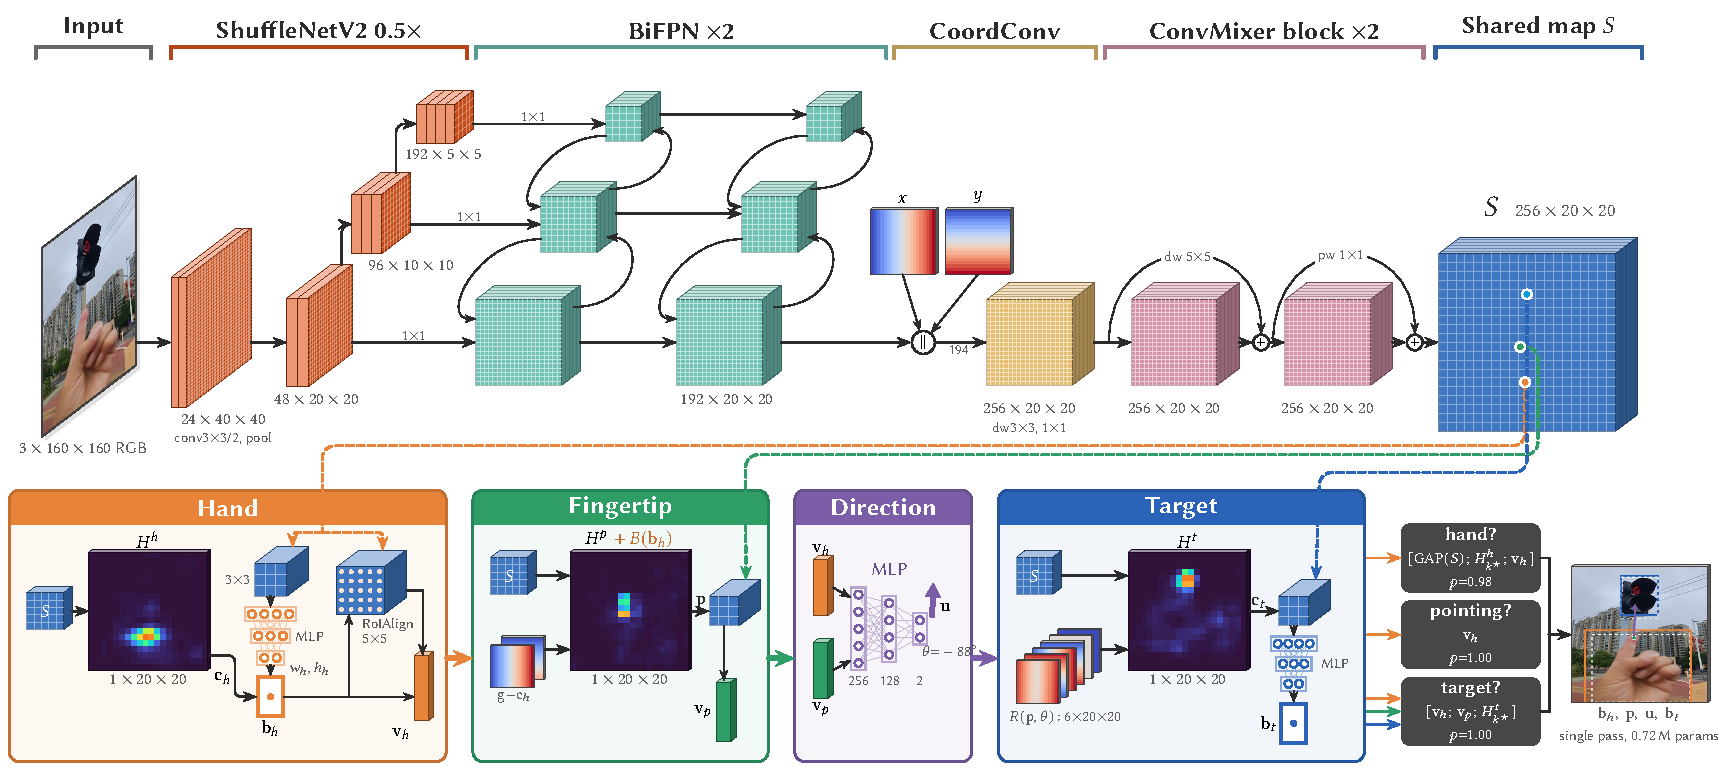
\includegraphics[width=\textwidth]{figures/architecture.pdf}
\caption{Compact instance-conditioned prediction. The hand, fingertip and target heads read the shared visual map at the previously predicted location (dashed). The selected hand supplies a box descriptor and fingertip-relative coordinates; hand and fingertip descriptors predict direction. A learned appearance-and-ray branch adds to the target heatmap, rather than restricting it to a hard cone. Local sampled features predict hand and target sizes. Distractor supervision is used only during training. The heatmaps are the trained model's outputs on one test image, overlaid on the frame and scaled to their maximum.}
\label{fig:architecture}
\end{figure*}

\subsection{Shared features and peak decoding}
A ShuffleNetV2 $0.5\times$ backbone provides stride-8, -16 and -32 features. Two bidirectional fusion layers produce 192 channels at stride 8. Depthwise smoothing with SimAM~\cite{yang2021simam}, coordinate channels and a projection to 256 channels precede two residual depthwise--pointwise mixing blocks. At 160-pixel input the shared map is $S\in\R^{256\times20\times20}$. This trunk combines local spatial detail with multi-scale context; individual component novelty is not claimed.

The hand, fingertip and target heads each predict a logit heatmap $h$. A global heatmap expectation can average distinct peaks into a location between instances. We instead take an expectation within a window $\mathcal W(k^\star)$ around the maximum-logit cell:
\begin{equation}
 \hat c=\sum_{k\in\mathcal W(k^\star)}
 \frac{\exp(\tau h_k)}{\sum_{j\in\mathcal W(k^\star)}\exp(\tau h_j)}\,g_k ,
 \quad k^\star=\arg\max_k h_k ,
 \label{eq:decode}
\end{equation}
where $g_k$ is a normalised grid coordinate. The hand and target use radius 2 and inverse temperature $\tau=8$; the fingertip uses radius 1 and $\tau=10$. Coordinates are continuous within the selected window. The discrete choice of window is not differentiable, although the expectation inside it is.

\subsection{From a hand instance to a target}
\paragraph{Hand and fingertip.}
The hand heatmap gives its centre. Bilinear sampling of a $3\times3$ neighbourhood of $S$ supports width and height regression. A $5\times5$ lattice over the predicted box, enlarged by 1.15, yields a 128-dimensional hand descriptor $v_h$. The fingertip heatmap combines a visual branch with a branch conditioned on hand-centre-relative coordinates. A soft logit penalty discourages fingertip locations outside the hand box enlarged by 1.3. The penalty uses detached box coordinates, so this prior does not push the hand box through its own gradient. A $3\times3$ neighbourhood around the decoded fingertip gives a second 128-dimensional descriptor $v_p$.

\paragraph{Direction and target.}
An MLP maps $[v_h;v_p]$ to a normalised vector $d=(d_x,d_y)$. Its target is the direction from the annotated fingertip to the annotated target-box centre, not a measured anatomical finger axis or a three-dimensional ray. This definition lets all required supervision come from the available annotation, but makes direction accuracy dependent on the chosen target extent.

The target heatmap combines visual evidence with learned spatial conditioning:
\begin{align}
 h^t_k &= V(S)_k+G([S;R(p,d)])_k, \label{eq:target}\\
 R_k &= (\Delta_x,\Delta_y,\Delta\cdot d,
              |\Delta_xd_y-\Delta_yd_x|,d_x,d_y), \nonumber\\
 \Delta &= \alpha(g_k-p). \nonumber
\end{align}
The scale $\alpha$ is learned. The final layer of $G$ starts at zero, so training begins with the visual branch alone. Both appearance features and ray-coordinate channels enter $G$; it is not a purely geometric prior. No hard constraint forces the target in front of the fingertip. The decoded target centre again anchors a $3\times3$ visual sample for box-size regression.

The hand gate receives pooled scene features, the hand heatmap peak and $v_h$. The pointing gate receives $v_h$, and the target gate receives $v_h$, $v_p$ and the target heatmap peak. At inference, sigmoid outputs are read as a cascade with threshold 0.5. This links confidence to the selected instance, but does not guarantee immunity to distractors.

\subsection{Training for localisation and ownership}
\paragraph{Localisation objective.}
Training sums masked losses for boxes, points, direction, heatmaps and gates. The hand uses CIoU~\cite{zheng2020distance}; the fingertip uses Wing loss~\cite{feng2018wing}; direction uses cosine error. The target objective combines IoU with SIoU-inspired distance and shape penalties~\cite{gevorgyan2022siou}, plus an auxiliary $1-\mathrm{IoU}$ term. The implemented distance penalty is a power of the normalised centre displacement, rather than the exponential distance term in canonical SIoU. Gaussian centre targets supervise heatmaps with a penalty-reduced focal objective, while focal binary cross-entropy supervises valid gate populations.

Two low-weight terms encourage consistency among predicted outputs. For $r=\hat c_t-\hat p$, the ray term is
\begin{equation}
 \mathcal L_{\rm ray}
 =\|r-(r\cdot\hat d)\hat d\|_2
   +0.5[-r\cdot\hat d]_+ .
 \label{eq:rayloss}
\end{equation}
The hand-axis term penalises $\max(0,0.5-\hat a\cdot\hat d)$, where $\hat a$ points from predicted hand centre to fingertip. It is a weak plausibility regulariser, not an assertion that the finger and target-centre directions always coincide. Section~\ref{sec:ablation} tests whether these losses actually improve the target box.

\paragraph{Distractor supervision.}
The released annotations do not provide positive labels for bystander hands. We therefore paste up to two hand crops into training images, keeping the original wearer/target labels. Crops may come from another image or the same wearer. Pasting is attempted with probability 0.5 on hand-positive and 0.3 on no-hand images. Scale changes and reorientation vary the appearance; crop centres are restricted to the upper 65\% of the image and overlap with labelled regions is limited. This encodes a useful but restrictive prior that the wearer hand usually enters from below.

Distractor boxes are retained to reweight negative hand-heatmap supervision. If $D_k$ is the maximum Gaussian response centred on a pasted hand, the negative weight is $1+4D_k$. The added hand is thus an explicit negative reference, even though it looks like a valid hand. This mechanism should be judged by whether localisation survives interference and whether a frame containing only other hands is rejected, rather than solely by whether a hand centre is selected correctly.

\paragraph{Optimisation and implementation.}
We use ImageNet backbone initialisation, AdamW~\cite{loshchilov2019decoupled}, batch size 32 and weight decay $10^{-4}$. A one-cycle schedule~\cite{smith2019super} peaks at $3\times10^{-3}$ for heads and $3\times10^{-4}$ for the backbone, with 10\% warm-up. Training permits 180 epochs and stops after 25 without improved validation loss; the selected checkpoint minimises that loss. Ground-truth centres replace predicted training anchors with probability 0.5, linearly decreasing to zero over 20 epochs. Other augmentations include horizontal flips, modest spatial and photometric transforms, and same-state image mixing that retains the dominant image's spatial labels. The 13 loss weights and exact target-loss definition accompany the source.

The full network has 722,104 parameters. At 160 pixels, PyTorch operation counting reports 0.231 GFLOPs with multiply--accumulate counted as two operations; unsupported operations, including bilinear sampling, are omitted. Serialised FP16 weights occupy approximately 1.6\,MiB. Weight storage and counted operations describe the model, not total runtime memory or end-to-end latency.
